\documentclass[border=6pt]{standalone}
\usepackage{tikz}
\usepackage[edges]{forest}
\usetikzlibrary{arrows.meta,positioning,calc,decorations.pathreplacing,shapes.geometric}
\begin{document}
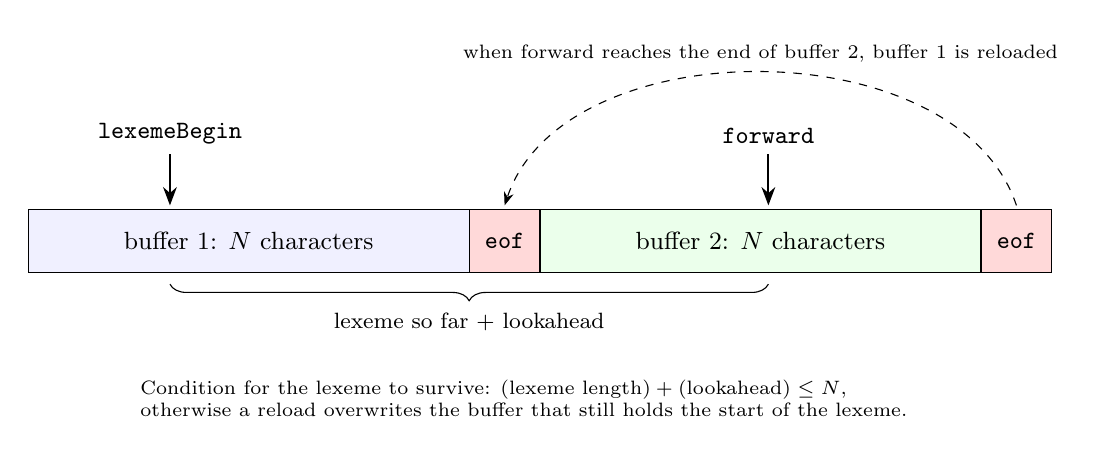
\begin{tikzpicture}[>=Stealth,font=\small,
 cell/.style={draw,minimum height=0.8cm,align=center}]
\node[cell,minimum width=5.6cm,fill=blue!6] (b1) at (0,0) {buffer 1: $N$ characters};
\node[cell,minimum width=0.9cm,fill=red!15] (e1) at (3.25,0) {\texttt{eof}};
\node[cell,minimum width=5.6cm,fill=green!8] (b2) at (6.5,0) {buffer 2: $N$ characters};
\node[cell,minimum width=0.9cm,fill=red!15] (e2) at (9.75,0) {\texttt{eof}};
\draw[->,thick] (-1.0,1.1) node[above] {\texttt{lexemeBegin}} -- (-1.0,0.45);
\draw[->,thick] (6.6,1.1) node[above] {\texttt{forward}} -- (6.6,0.45);
\draw[decorate,decoration={brace,amplitude=6pt,mirror}] (-1.0,-0.55) -- node[below=7pt,font=\footnotesize] {lexeme so far $+$ lookahead} (6.6,-0.55);
\draw[->,dashed] (9.75,0.45) .. controls (9.0,2.7) and (4.0,2.7) .. node[above,font=\scriptsize,pos=0.5]{when forward reaches the end of buffer 2, buffer 1 is reloaded} (3.25,0.45);
\node[font=\scriptsize,align=left,anchor=west] at (-1.5,-2.0) {Condition for the lexeme to survive: $(\mathrm{lexeme\ length}) + (\mathrm{lookahead}) \le N$,\\otherwise a reload overwrites the buffer that still holds the start of the lexeme.};
\end{tikzpicture}
\end{document}
